Tunable light sources image loaded by the function \texttt{load\_tunable\_image} in Code \ref{code:load--tunable} is saved in the ENVI format.
The script for saving the image is shown in Code \ref{code:save-tunable}.
The spectral image is saved as a raw file with the BIL interleave. 

Preview by FreeLook software is shown in Figure \ref{fig:tunable-preview}.
\begin{figure}[H]
    \centering
    \caption{Preview of the Tunable light source image in FreeLook software}
    \label{fig:tunable-preview}
    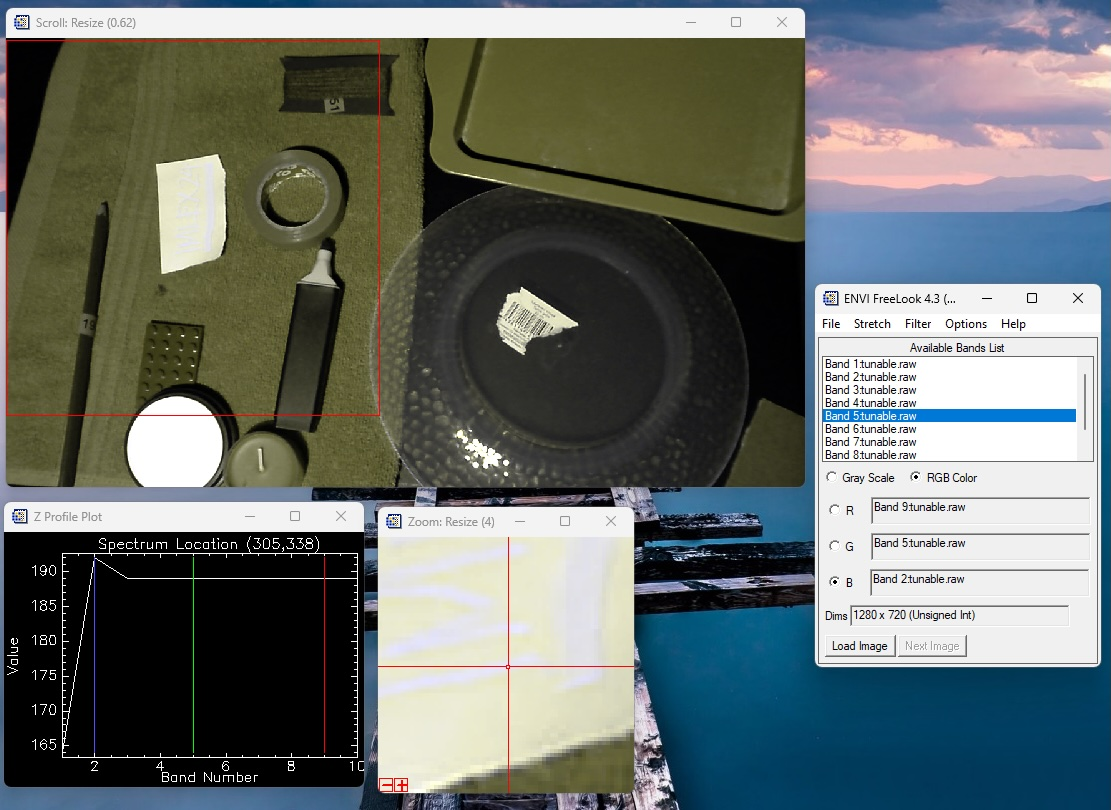
\includegraphics[width=0.5\textwidth]{./fig-task3/tunable.jpg}
\end{figure}

The header file is shown in Code \ref{code:tunable-hdr}.

\begin{lstlisting}[caption=Saved ENVI header file, label={code:tunable-hdr}]
ENVI
ENVI description = {File Imported into ENVI}
file type = ENVI
lines = 720
samples = 1280
bands = 10
interleave = bil
data type = 12
header offset = 0
byte order = 0

\end{lstlisting}